\documentclass[a4paper, top=10mm]{article}
%for writing from the top
\usepackage{fullpage}
%for math
\usepackage{amsmath}
\usepackage{mathrsfs}
\usepackage{amsthm}
%for images
\usepackage{graphicx}
%for color
\usepackage{xcolor}
%for title
\title{\textbf{\huge{Christmas Marble}}}
\author{Enigma n\textsuperscript{o}1}
\date{19\textsuperscript{th} December 2024}

\newtheorem*{hint}{Hint}

\addtolength{\voffset}{-2cm}
\addtolength{\textheight}{5cm}


\begin{document}
	\maketitle
	
	It was the holiday season, and Gabriel (artistic director of the MICS) had taken on the joyful task of decorating the lab’s Christmas tree.
	This wasn’t just any tree—it was a masterpiece of creativity, blending festive cheer with scientific flair.
	
	Among the decorations was a large, pristine Christmas ball, gleaming like a star under the lab’s bright lights.
	But Gabriel, ever the innovator, decided it needed a touch of science-inspired artistry.
	
	“Let’s give this ball a unique twist,” he announced to the curious lab members watching him work. With a steady hand and a precise drill borrowed from the "Fabrique" (fablab downstairs), Gabriel carefully bored a cylindrical hole straight through the center of the Christmas ball.
	
	Once the transformation was complete, Gabriel placed the modified ornament on the lab bench for everyone to admire. The pierced ball stood upright, its height from the table measuring exactly 10 cm.
	
	As the team marveled at his creation, a challenge emerged:
	
	“Gabriel, how much of the original volume remains after the hole is drilled?”
	
	Gabriel grinned and replied, “That’s for you to figure out! Consider it a festive puzzle—combine your holiday spirit with your scientific skills.”
	
	Can you solve the mystery and calculate the remaining volume of Gabriel’s drilled Christmas ball?\\
	\textit{Give your answer in $mm^3$ rounded to the closest integer.}
	
	\begin{center}
		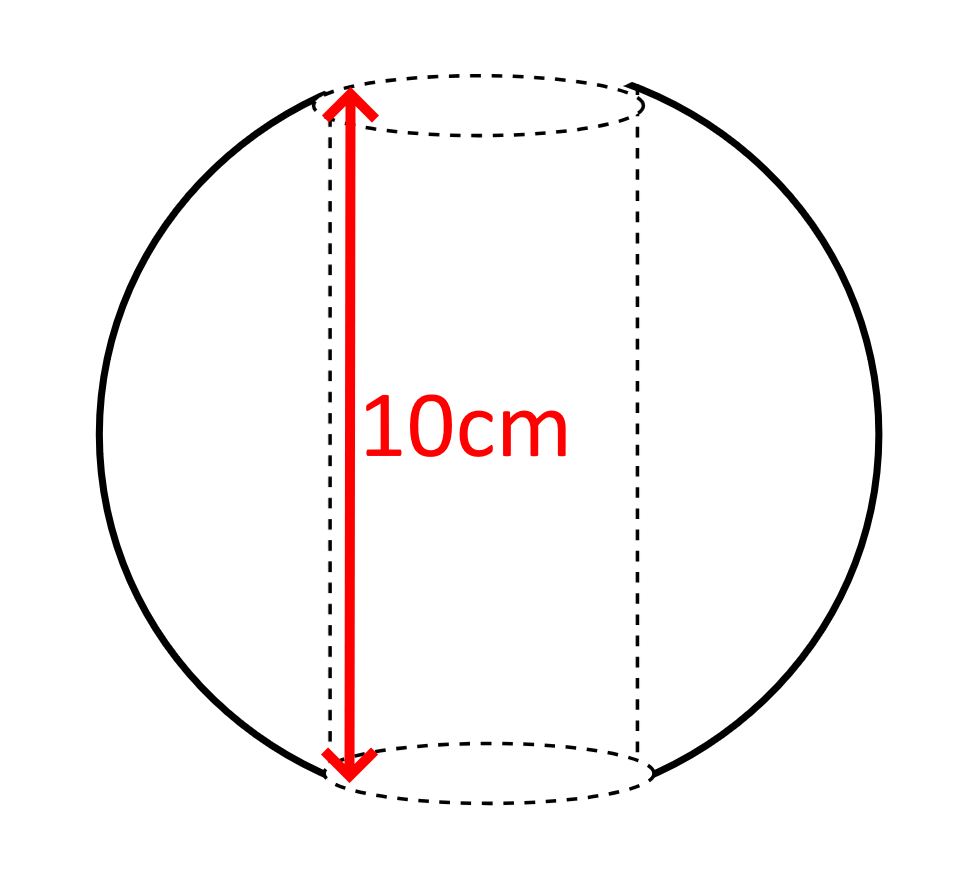
\includegraphics[height=200pt]{01xmas_pearl.png}\\
		Diagram of the Christmas marble.
	\end{center}
	
	\underline{Hint 1:} Use cylindrical coordinates, and $dV = r\ dr\, d\theta\, dz$.\\
	
	\underline{Hint 2:} No, you are not missing any information to be able to answer!
	
% Answer:
% 523.598775598 cm^3 => 523599 mm^3
% full explaination:
% https://www.sfu.ca/~adebened/funstuff/sphere_cyl.pdf
	
\end{document}